\documentclass[letter]{article}

\usepackage{MD_estilo}

\nombre{Vicente Vial} % Aqui va el nombre del alumno
\numtarea{10} % Aqui va el número de la tarea

\sigla{IIC2343} % Aqui va la sigla del curso
\curso{Arquitectura de computadores} % Aqui va el nombre del curso
\semestre{2} % Aqui va el semestre del curso
\ano{2018} % Aqui va el año del curso


\begin{document}
	
	\begin{pregunta}{1} % Aqui se coloca el número de la pregunta
	
	FUENTE: EXAMEN 2015-2 PREGUNTA 1
	$$ $$
	a) No se sabe a ciencia cierta que va a ocurrir, lo más probable es que los opcodes difieran, luego si se intenta ejecutar el código y el sistema no lo prohibe,no se podrá saber con certeza que ocurrirá , y será imposible predecir como se comportará el computador. 
		$$ $$
	b) Lo que hace el disassembler es convertir el código binario(instrucciones) en un código assembly, para esto va identificando cada opcode según las tablas de opcode entregadas, esto se puede hacer debido a la estructura de los opcodes, para el caso de 2 opcodes el disasembler debería poder identificarlos, estos opcodes los a convirtiendo en el lenguaje assembly según la tabla de opcodes. Para el caso de los literales, se pueden identificar fácilmente por la estructura de los opcodes.
	
	No se puede obtener el assembly original a partir de un programa ubicado en la memoria de instrucciones, debido a que los labels se pierden.
	
	
	
	$$ $$
	
	
	
	c) Mecanismo para generar un archivo ejecutable en x86, a partir del resultado de un assembler para el computador básico:
	
	1º) Disassembler generar assembly del computador básico, a partir del código ejecutable guardado en la memoria de instrucciones.
	
	2º)Se convierte el assembly generado anteriormente en assembly en x86. Para esto se hace lo siguiente:
	(El assembly corresponde a un computador de 16 bits, por lo que se puede hacer los siguientes pasos)
	
	a) Registro A se cambia a AL
	
	b) Registro B se cambia  BL
	
	c) Se copia contenido de variables declarada después de las instrucciones en el código assembly(cada vez que se requiera usar el contenido de memoria, se tiene que transoformar esta dirección en la nueva ubiación)
	
	3º) Código assembly x86 se procesa con un assemble x86, para generar el código ejecutable.
	
	
	
	
	
	
	
	
	
	
	
	
	\end{pregunta}
	
	\begin{pregunta}{2}
	FUENTE: SOLUCIÓN I1 2011`2
$$ $$
	
a)  Lo almacenariá en una matriz (de 5 columnas y 5 columnas)que usa secuencia de filas,  donde cada elemento tiene 2 palabras.
$$ $$
b)	La dirección del elemento i,j será la siguiente:

$$dir(matriz[i,j]) = dir(matriz) + i*sizeof(matriz[i,j])*columnas + j * sizeof(matriz[i,j])$$
Como (1,1) corresponde a las cordenadas del pixel superior izquierdo, y se cuenta con 5 columnas,  sizeof(matriz[i][j]) = 2, y que dir(matriz) = 0x6E la posición 3,4 se encuentra en:
$$dir(matriz[3,4]) = 0x6E + (i-1)*2*5 + (j-1) * 2$$
$$dir(matriz[3,4]) = 0x6E + 2*2*5 + 4* 2$$
$$dir(matriz[3,4]) = 136$$

$$ $$

c) Almacenaría la imagen, de una manera similar pero ahora cada elemento tendrá 3 palabras(1 por cada color), entonces, para almacenar la imagen, usaría una matriz (de 7 columnas y 7 filas) que usa secuencia de fila, donde cada elemento tiene 3 palabras.

$$ $$

d) Una imagen de color 7x7 pixeles y 2 byte, necesita $$7X7X3X2 bytes = 294 bytes$$
y la memoria tiene sólo 256 bytes, se puede solucionar con una memoria de mayor tamaño, donde haya una mayor cantidad de palabras posibles.
$$ $$
e)Adaptando lo que tenía anteriormente, la fórmula es la siguiente:
$$ dir(img[i,j,k])=dir(img)+i*sizeof(img[i,j,k])*3*cols+
j*sizeof(img[i,j,k])*3+k*sizeof(img[i,j,k])$$

\end{pregunta}
	
	\begin{pregunta}{3}
	a) Los bits de paridad se utilizan para detectar   errores al transmitir información binaria. Para esto se utiliza un bit adicional, el cual se utiliza para que siempre haya una cantidad par de 1. 
	$$ $$
    b) Pueden haber distintos casos, si es que se sabe de donde viene la información se podría solicitar nuevamente el ingreso de la información, si no se sabe de donde viene la información, se podría marcar la posición actual de la memoria para que no se tome en cuenta al correr el programa y de alguna manera notificar que la palabra tenia un error, ó se podría reemplazar la variable en esa posición por una variable neutral. El gran problema, es que el computador sólo podrá detectar que hay un error, pero no sabrá cual es el error, por lo que no puede arregar el problema por su cuenta.
    
    $$ $$
    
    c)
    $$ $$
    {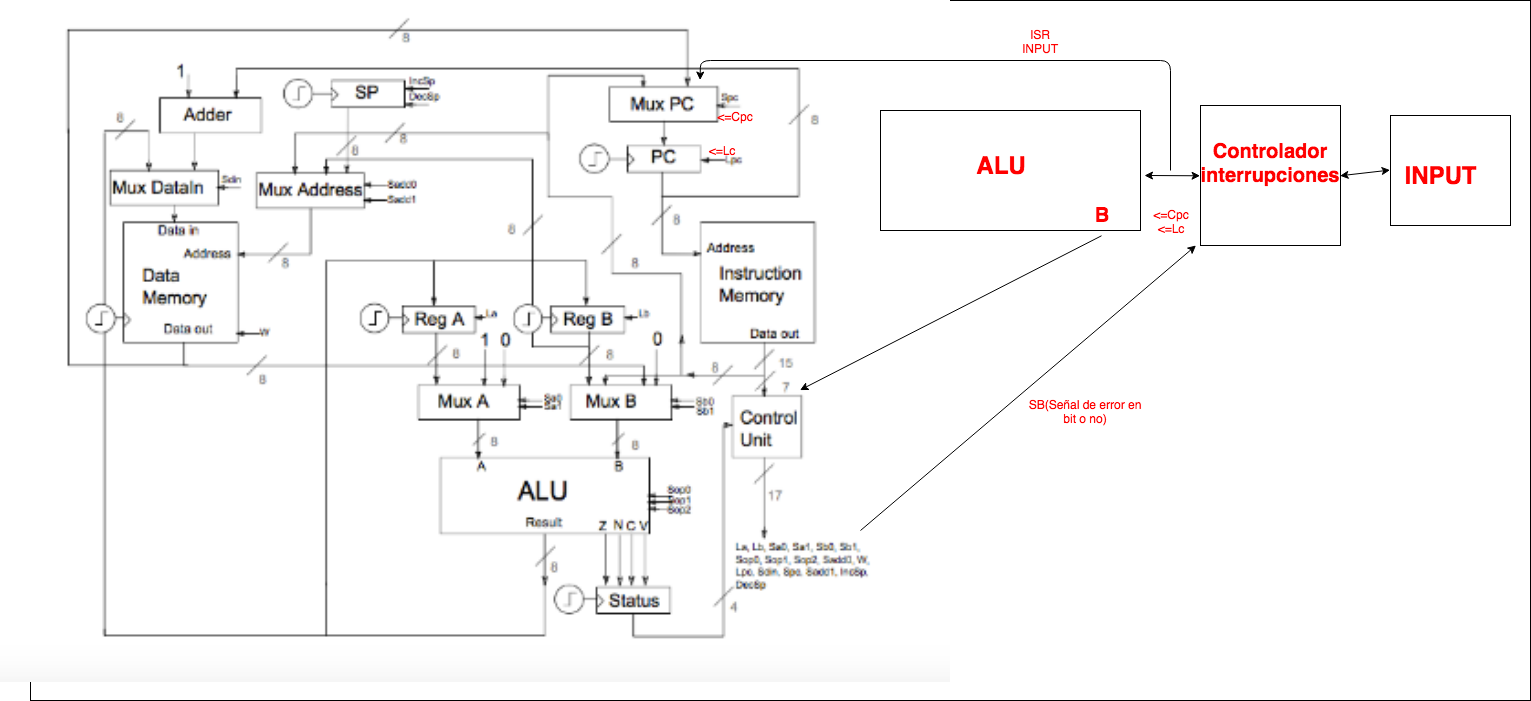
\includegraphics[width=15cm]{arquitectura.png}}
     $$ $$
    La idea es la siguiente, se tiene el input y el controlador de interrupciones, este funciona normalmente con sus señales respectivas(las omiti en la imagen por un tema de orden), el controlador de interrupciones enviará el ISR al MUX PC, y se enviará la señal CPC para que se seleccione, y luego la señal LC para que se cargue en el PC. A la par, el ISR se manda a la ALU(ALU en rojo), y esta comprueba si el código del bit de paridad es erroneo o no(resultado B) ,y manda un bit al control unit indicado el estado de la comparación. El control Unit recibe este bit junto con el Data Out de la ROM, y según eso manda las señales correspondientes, si el bit indica error, bloquea todas las señales y manda un aviso al controlador de interrupciones para que mande denuevo la información, si esta bien la comparación, manda las señales de forma normal.
    $$ $$
    
    d) Uno de los  factores que limita la velocidad de transferencia sería tiempo que demora la revisión de el bit, pasando por nuevas compuertas binarias lo que retrasa la ejecución. También otro factor que retrasa es cuando existe un error en la transferencia, ya que se tiene que pedir nuevamente la información, realizar el proceso denuevo y bloquear las señales.
    
    
	\end{pregunta}

	\begin{pregunta}{4}
	$$ $$
	a) ¿Qué ventajas le entrega este diseño respecto a una maquina de registros?
	Las ventajas es que los códigos de operación son más simples y  fáciles de escribir compiladores. Además, los códigos tienen una mejor densidad de código. También el manejo de los datos se hace en memoria, y las instrucciones no se tienen que referir a registros, sino que se van seleccionando las variables desde el stack, lo que hace más fácil la escritura. Es un modelo más sencillo para la evaluación de expresiones. Y es más fácil adaptar el código a distintos computadores.
	$$ $$
	b) La principal desventaja para el usuario es la disminución de la velocidad del sistema por usar stack, ya que que el stack interactúa constantemente con la memoria, y la memoria es más lenta que los registros de la CPU en una variedad de formas. Por lo general, tiene una latencia más larga y un ancho de banda menor. Los accesos a la memoria son más difíciles de acelerar. Incluso en un procesador muy simple, el acceso a la memoria puede tomar un ciclo adicional o más en comparación con el acceso al registro. El acceso al registro es efectivamente instantáneo en la mayoría de los casos, mientras que el acceso a la memoria toma al menos un ciclo. Todo esto repercute en un sistema que demora más, lo que influye negativamente en el usuario.
	$$ $$
	c)  Si es posible crear un chip que cumpla las  especificaciones de la JVM, esto ya que primero por la experiencia cotidiana vemos que podemos usar en nuestro computador, máquinas de stack virtuales. Luego, para que un chip cumpla las especificaciones, tiene que poder ejecutar el JVM, para eso tiene que tener ciertas consideraciones con el uso del stack, y podrá implementarse correctamente. El stack lo que hace es que va a agregando y desechando palabras constantemente, un chip puede cumplir con esos requerimientos pero debe tener ciertos criterio para eliminar las cosas menos importantes o con menos uso, según estime el programador. Luego, el chip funcionará correctamente, cumpliendo las especifaciones de JVM. (FUENTE: pdfs.semanticscholar.org)
	
	
		
	\end{pregunta}


	\begin{pregunta}{5}

	
	
	FUENTE: Prueba I2 2012-1 PREGUNTA 3
	
	$$ $$
		a)
	
	Los cambios presentados añaden 8 nuevas instrucciones al computador,cada de una de ellas esta relacionada con los cambios pedidos. Estas instrucciones toman los valores de los registros A y B, los cambian de acuerdo a la operación y al literal ingresado como parámetro, y luego los almacenan nuevamente en los registros A y B. Desde el punto de la microarquitectura, se agrega una ALU adicional, cuyo output se conecta al registro B, por medio del nuevo MUX B2. Además, se agrega la nueva señal Sb2, que controla al MUX B2.
La siguiente figura muestra sólo lo que se cambio en el computador básico, todo los demás sigue igual:
	$$ $$
	 {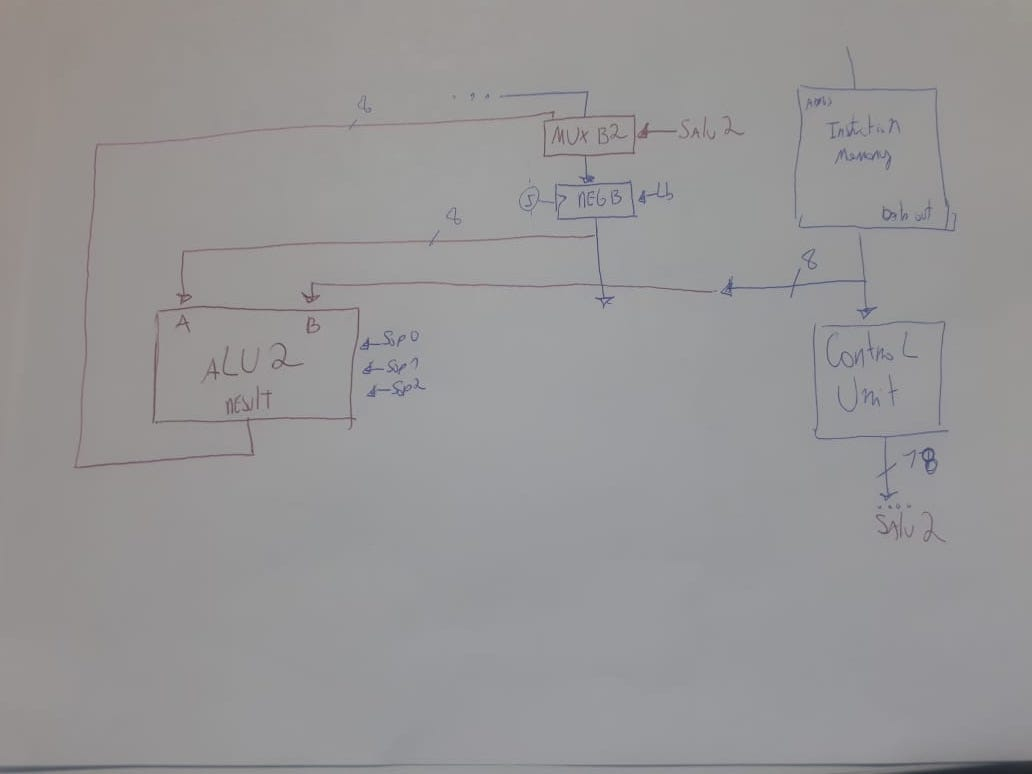
\includegraphics[width=15cm]{p1.jpeg}}
	$$ $$
La siguiente tabla presenta los opcodes y señales de control de las nuevas operaciones,excluyendo las señales que se repiten en todas las operaciones( Sadd=-, Sdin=-, Spc=-, W=0, IncSp=0 y DecSp=0.)
$$ $$
{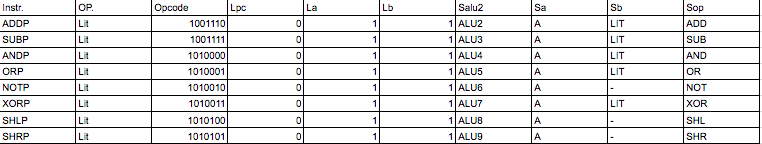
\includegraphics[width=15cm]{tabla2.png}}
	\end{pregunta}


$$ $$
	b)El cambio realizado modifica la memoria ROM de instrucciones por una memoria RAM, para que pueda ser escrita. Además se añade un mux (Mux Address 2) para elegir el origen de la dirección que ingresa a la memoria(PC ó dirección obtenida de Mux Adrres). Para estar seguro de  que la instrucción siguiente a la de escritura se ejecute de buena manea, se añade una nueva señar al PC, HaltPC, que evita que este se incremente por una iteración. También se añade la instrucción NOP, que causa que el computador no haga nada por un ciclo y se agrega un enabler (NOPEn) a la salida de la memoria de instrucciones, que al ser activado con  W1=1, evita que pase la instrucción actual y genera el opcode de la nueva instrucción NOP, mientras que si no es activado, es decir en W = 0, deja pasar el opcode ingresado. Finalmente, los datos de entrada para esta memoria se obtienen desde la ALU. La figura muestra el computador sólo con sus partes modificadas, el resto sigue igual:
	
$$ $$

{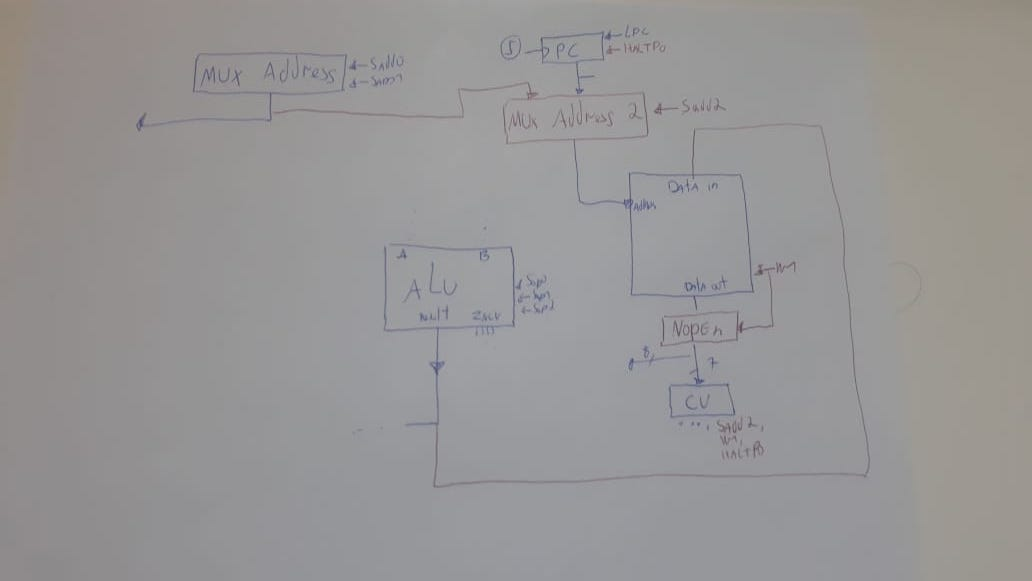
\includegraphics[width=15cm]{arqui2.jpeg}}

$$ $$

En la  ISA, además de NOP, se agregan las instrucciones MOV DM (Dir),
A y MOV DM (B), A, que escriben el valor almacenado en el registro A en la memoria de datos.
Estas instrucciones toman 2 ciclos, una para escribir el dato en memoria y la siguiente ejecutando NOP. Las siguientes tablas presentan los opcodes y señales de control de las nuevas instrucciones, incluyendo las nuevas señales Sadd2, HaltPc y W1:


$$ $$
{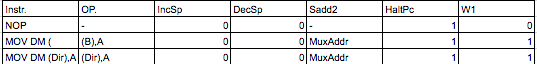
\includegraphics[width=15cm]{graf2.png}}
$$ $$
{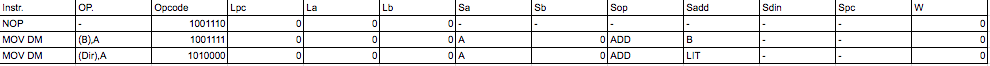
\includegraphics[width=15cm]{graf1.png}}

$$ $$

c) La microarquitectura definida es la siguiente:

$$ $$
{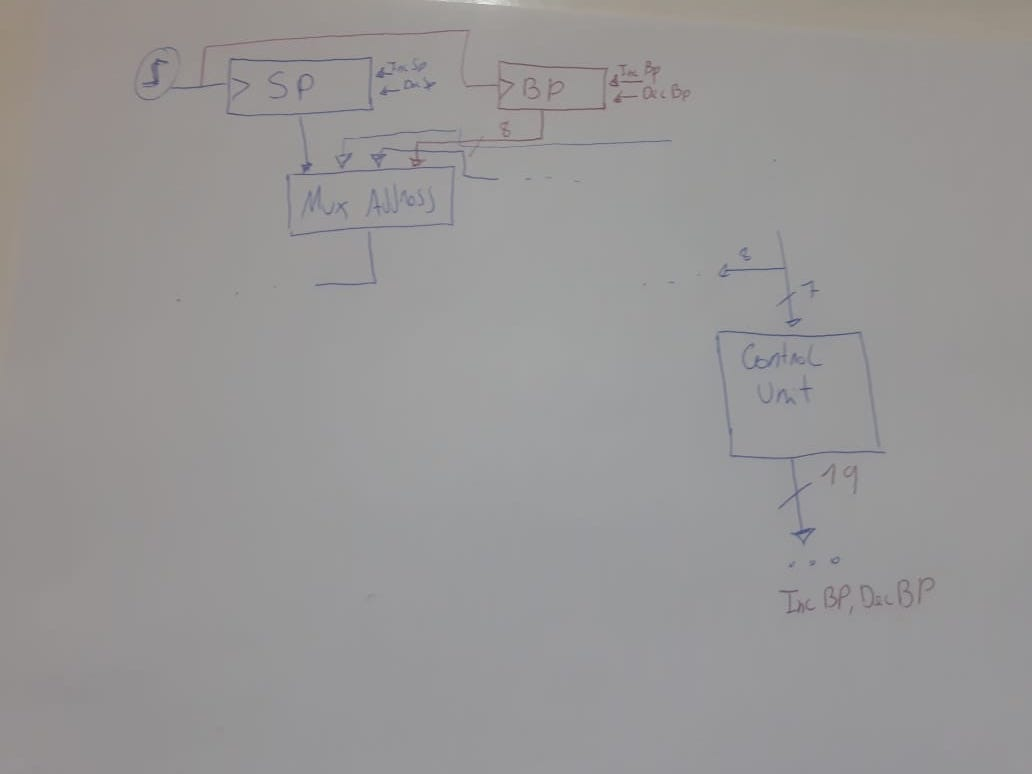
\includegraphics[width=15cm]{p3.jpeg}}
$$

d) La microarquitectura definida es la siguiente:

$$ $$

{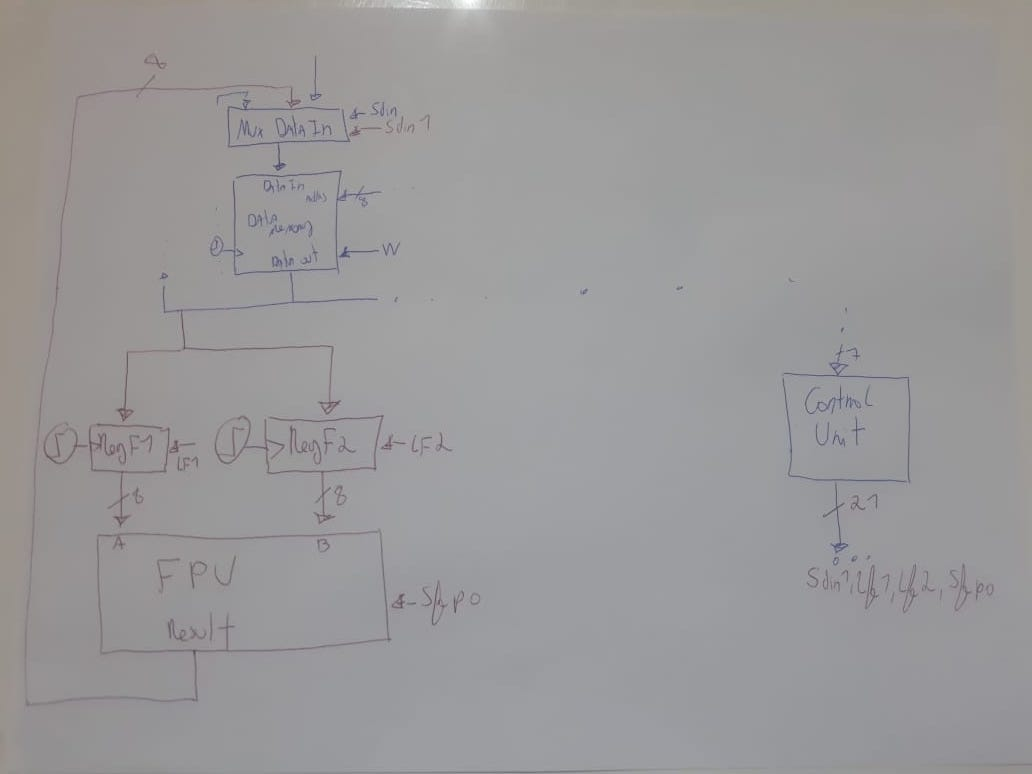
\includegraphics[width=15cm]{p4.jpeg}}

\end{document}